\section{Background}
\label{sec: background}

In this section, we offer some background information relevant to our study, focusing on the concurrency control protocols used by the evaluated systems and the important aspects of the PPS workload used in our benchmark.

\subsection{Evaluated Database Systems}
This study evaluates five geo-distributed database systems: Detock, SLOG, Calvin, Caerus, and Mencius. Each system has its own deployment strategy and has a distinct approach when it comes to handling concurrent transactions.

Among these, Detock, SLOG, and Calvin are based on \textit{deterministic scheduling}, a recent alternative to traditional protocols that use atomic commitment \cite{thomson2010case}. These deterministic database systems avoid the need for runtime coordination between different servers by predefining the execution order of transactions. This design reduces the communication overhead, particularly in the context of inter-region delays. However, these systems face challenges when handling \textit{dependent transactions}, namely transactions for which the complete read/write sets are not known in advance. The three deterministic systems we consider are:
\begin{itemize}
    \item \textbf{Calvin}: It was the system that demonstrated the feasibility of deterministic transaction processing at scale \cite{thomson2012calvin}. The system works by using short epochs to batch the received transactions and using \textit{global sequencers} to collect and order them.
    \item \textbf{SLOG}: It was built on top of Calvin by optimizing for data locality when used in geo-distributed settings. It introduces the notion of \textit{single-home transactions} that access data in a single region, and thus can be processed with very low latency without being passed to the global ordering layer \cite{ren2019slog}.
    \item \textbf{Detock}: It is also based on Calvin's architecture, but it removes the need for global ordering by using a deadlock resolution protocol via a \textit{dependency graph} \cite{nguyen2023detock}.
\end{itemize}
[TODO: Caerus and Mencius]

\subsection{Product-Parts-Supplier Workload}
The PPS workload simulates a realistic supply chain management, capturing the interactions between products, their composing parts, and the suppliers that provide those parts. Figure~\ref{fig: pps-erd} shows the relational schema of the PPS workload. 

\begin{figure}
    \centering
    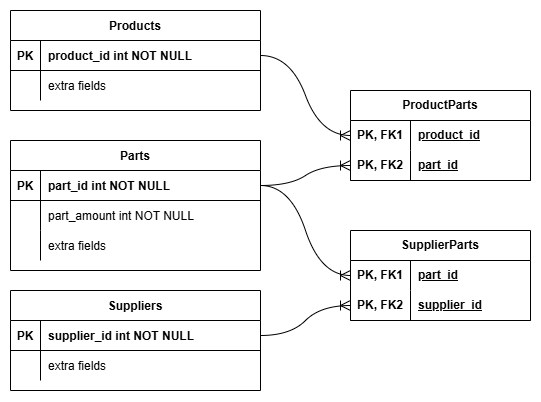
\includegraphics[width=1\linewidth]{figures/PPS ERD.png}
    \caption{Product-Parts-Supplier Entity Relationship Diagram}
    \label{fig: pps-erd}
\end{figure}

This workload reflects complex transactional dependencies often found in enterprise applications such as large-scale inventory management. PPS is composed of several types of transactions, including:
\begin{itemize}
    \item \textit{OrderProduct}: It decrements the inventory amount of the parts associated with the given product. 
    \item \textit{GetPartsByProduct}: It retrieves the list of parts that compose a given product.
    \item \textit{UpdateProductPart}: It modifies the relationship between a product and its associated parts.
    \item \textit{GetPart}: It is a simple lookup that fetches the current inventory amount of a specific part, along with any additional information.
    \item \textit{GetProduct}: It retrieves the existing extra information about a given product.
\end{itemize}

